\documentclass[sigconf]{acmart}

%% Suppress ACM reference format and copyright footer for class use
\settopmatter{printacmref=false}
\renewcommand\footnotetextcopyrightpermission[1]{}
\pagestyle{plain}

\usepackage{graphicx}
\graphicspath{{figures_new/}{figures/}}

\begin{document}
\title{Programmable Criticality-Aware Object Placement Across Tiered Memory in OCaml~5}

\author{Andrew Li}
\affiliation{%
  \institution{Northwestern University}
  \city{Evanston}
  \state{IL}
  \country{USA}
}
\email{andrewli@u.northwestern.edu}

\begin{abstract}
Data-intensive workloads are increasingly bottlenecked on DRAM capacity,
motivating heterogeneous memory hierarchies in which local DRAM is augmented by
cheaper, slower ``far memory'' tiers such as CXL-attached memory. OS-level
paging is blind to application object structure and so places memory poorly;
recent work argues for \emph{criticality}-based placement that accounts not just
for hotness but for memory-level parallelism (MLP). Only the language runtime
knows enough about object structure to make these decisions well. We present a
framework for \emph{programmable} garbage-collector object placement across
tiered memory in OCaml~5 --- in effect \emph{\texttt{sched\_ext} for GC
placement}. The runtime supplies all mechanism (arenas, promotion, pointer
fixup, fact collection); a user-supplied \emph{policy} --- a single pure C
function, loaded as a built-in or \texttt{dlopen}'d \texttt{.so} --- supplies
only judgment: given cheap facts about one object, which tier should it live in.
We additionally thread \texttt{[@far\_memory]}/\texttt{[@main\_memory]} source
attributes through the compiler so programmers can place objects by hand. On an
emulated CXL device (far memory $4.6\times$ higher access latency and
$\sim\!4.5\times$ lower read bandwidth than DRAM), the framework adds no
measurable overhead over stock OCaml, a placement decision costs $\sim\!2$~ns
(the \texttt{dlopen} indirection adds only a few tenths of a nanosecond), and
under a DRAM cap at half the working-set footprint a criticality-aware policy
recovers most of the all-in-DRAM performance while a naive all-far placement is
up to $2.4\times$ slower.
\end{abstract}

\keywords{OCaml, garbage collection, far memory, CXL, tiered memory, object placement}

\maketitle

\section{Background}

Data-intensive workloads consume large quantities of DRAM, which is increasingly
expensive given the growth of AI data centers. This memory bottleneck motivates
a transition to heterogeneous memory hierarchies, where local DRAM is augmented
by cheaper ``far memory'' tiers like Compute Express Link
(CXL)-attached memory~\cite{cxl2024}. Traditional OS-level paging lacks insight
into application object structure, leading to suboptimal placement of objects
into pages across memory tiers. Heuristically it may seem reasonable to place
objects by hotness or access frequency~\cite{merchandiser2023}, but recent
research has shifted toward criticality-based paging, which uses not just hotness
but also memory-level parallelism (MLP). The intuition is that some data
structures are friendly to hardware-level parallel access while others ---
pointer-chasing structures in particular --- are not, so that the same access
frequency can hide very different amounts of latency. The OS understands none of
this; only language runtimes do. Managed runtimes with garbage collection (GC)
already relocate objects freely, and this object mobility is a fundamental
advantage of managed over unmanaged languages~\cite{alaska2024}. OS-level
frameworks such as PACT, with its Per-page Access Criticality
metric~\cite{pact2026}, are necessarily blind to the runtime's structural
knowledge.

\section{From a heuristic to a framework}

The original proposal for this project aimed to discover \emph{the} winning
runtime-level criticality heuristic and bake it into the OCaml GC. Three
weaknesses doomed that framing: criticality metrics are genuinely hard to
engineer; even good metrics are hard to find and validate; and a single baked-in
heuristic is hard to review and easy to get subtly wrong. We therefore pivoted.

The contribution of this work is the \textbf{framework}, not any one heuristic.
We build a strict \emph{mechanism/policy split} --- in spirit, \texttt{sched\_ext}
for GC placement. The runtime (the ``engine'') owns all mechanism: when GC runs,
arena mapping, pool freelists, promotion atomicity, pointer fixup, thread
coordination, the computation of cheap per-object \emph{facts}, and --- crucially
--- the defense of heap correctness. A \emph{policy} owns exactly one thing: the
decision \texttt{features}~$\rightarrow$~\texttt{arena}. The headline results are
therefore \emph{expressiveness} (many distinct policies are expressible, tiny,
across three authoring surfaces) and \emph{overhead} (the framework hosts them at
near-zero cost), rather than ``our heuristic wins.'' Whether any particular
policy wins is then an empirical question the framework lets us ask cheaply.

We target OCaml~5~\cite{ocaml5gc2020} because its multicore, concurrent GC makes
the placement plumbing genuinely hard (placement decisions fire mid-collection,
concurrently across domains), and because its generational, copying minor heap
already promotes live objects to a major heap --- a natural seam at which to
choose a tier.

\section{Design}

\subsection{Mechanism/policy split}

Calls go one direction only: \textbf{engine~$\rightarrow$~policy}. The policy is
a passive callback table; it may never re-enter the runtime. The engine fills a
\texttt{caml\_placement\_features} struct on its own C stack and calls
\texttt{choose\_arena(const features*)}; the only value flowing back is an
\texttt{int} arena id. There is no serialization, no IPC, and no copy --- the
policy \texttt{.so} is \texttt{dlopen}'d into the same address space and shares
an identical struct layout guaranteed by a single header,
\texttt{runtime/caml/placement.h}. A one-time back-channel,
\texttt{features\_needed}, read once at \texttt{init}, lets a policy declare
which non-free facts are worth computing, so policies that do not want an
expensive fact never pay for it.

\subsection{The policy contract: a pure function}

The entire contract is one sentence: \texttt{choose\_arena} is a \emph{pure
function} of its \texttt{features} argument plus immutable configuration read at
\texttt{init} --- no mutable state, no domain-local scratch, no atomics. This
single constraint buys a great deal:

\begin{itemize}
  \item \textbf{No concurrency protection.} \texttt{choose\_arena} runs
  concurrently across domains during stop-the-world minor GC, but a pure
  function under concurrent calls has nothing to race on --- no locks, no
  reentrancy hedging.
  \item \textbf{History for free.} A policy that wants aggregate history reads it
  from the \texttt{arena\_used[]} snapshot the engine already places in
  \texttt{features}; it maintains nothing itself.
  \item \textbf{Determinism is not load-bearing for correctness.} Under the
  promotion race, several domains may speculatively place the same object; a
  compare-and-swap picks one arbitrary winner and the losers abandon their
  copies. The heap is correct regardless of which arena the winner chose. A pure
  function of an object's immutable features happens to be deterministic too,
  which is convenient for reproducibility, but integrity does not depend on it.
\end{itemize}

The callback fires mid-collection, while the heap is in an inconsistent
intermediate state (forwarding pointers, in-progress headers, the minor heap
being drained). Running OCaml there would allocate and could trigger a nested GC,
corrupting the heap. The callback is therefore \textbf{non-allocating C}. OCaml
authoring is still available, but safely: via source attributes (below), and a
deferred pure-expression DSL.

\subsection{The data model}

The engine fills a \texttt{caml\_placement\_features} record per object. We
populate a \emph{Tier-0} set of facts that are essentially free because the
engine already has them in hand at the promotion site --- among them the object's
size in words (\texttt{wosize}), its \texttt{tag}, a \texttt{scannable} bit
(1~=~pointer-bearing, a free \emph{low}-MLP proxy; 0~=~flat/\texttt{No\_scan}, a
free \emph{high}-MLP proxy), the compiler \texttt{hint} read from reserved header
bits, the allocating domain, minor-heap occupancy, and the live-words-per-arena
snapshot. Higher tiers --- structural facts (\texttt{fanout},
\texttt{chain\_depth}), write counts, allocation-site provenance, and PEBS-sampled
read hotness --- are present in the struct but zero, gated behind
\texttt{features\_needed} flags, so they can be enabled later with no ABI break.

The policy returns its descriptor through one exported symbol:

\begin{quote}\small\ttfamily
const caml\_placement\_policy\_ops *\\
\hspace*{1em}caml\_placement\_policy\_entry(void);
\end{quote}

\noindent
The descriptor carries an \texttt{abi\_version}, a \texttt{name},
\texttt{features\_needed}, and the callbacks (\texttt{init}, the required
\texttt{choose\_arena}, optional \texttt{after\_minor} telemetry, a reserved
\texttt{should\_migrate}, and \texttt{shutdown}). The ABI is append-only: new
fields go before a reserved tail, existing offsets never move, and a new feature
flag is just a new bit that old policies do not set --- so the engine skips that
work and they pay nothing. The version is bumped only on a layout-breaking
change, and the load-time check then refuses a stale \texttt{.so} with a clear
error rather than crashing.

\subsection{Registration and loading}

A single environment variable, \texttt{CAML\_GC\_POLICY}, is resolved at GC init
before domains spawn. A value containing a slash or ending in \texttt{.so} is
\texttt{dlopen}'d and its entry symbol resolved; otherwise the name is looked up
in a static built-in table; unset falls back to \texttt{all\_dram}, a
single-arena policy that behaves exactly like stock OCaml --- the safe baseline.
The active descriptor lives in a read-mostly global, set once and read lock-free
on the hot path. The user's compiled OCaml program is byte-for-byte identical
regardless of policy: loading happens in the runtime at process start, decoupled
from compilation.

\subsection{Two arenas}

The foundation is a behavior-preserving refactor of the shared-heap pool
allocator so that all existing allocation flows through arena~0 (DRAM); the full
testsuite gates this risky change. A second arena (far) is then mapped and, where
available, bound to a far-memory device, with graceful fallback to a plain
mapping where no such device exists --- so the whole framework is testable on any
machine, and a far-memory device is needed only for the performance numbers. As
the proposal anticipated, far memory is emulated not by injected latency in the
runtime but by the device topology of the host. The promotion path fills Tier-0
\texttt{features}, calls the policy, and routes the object to the chosen arena,
falling back to the other arena if the chosen one is full so the no-fail
promotion invariant is preserved.

\subsection{Compiler attributes}

For manual placement we thread two source attributes,
\texttt{[@far\_memory]} and \texttt{[@main\_memory]}, through the entire compiler
pipeline. They are registered as known built-in attributes (so no spurious
warning), threaded through the Lambda IR by extending \texttt{Pmakeblock} to
carry a memory hint, and lowered through Clambda/Cmm so the allocation's
\texttt{reserved} header argument is set on the minor-heap fast path. The GC then
reads the hint from the object header at promotion time. The tree is configured
with \texttt{--enable-reserved-header-bits=2} so that the baseline and attributed
conditions share one ABI and the comparison is fair. The built-in
\texttt{attribute} policy honors the hint (\texttt{FAR}~$\rightarrow$~far,
\texttt{MAIN}~$\rightarrow$~DRAM) and defers to a configurable sub-policy for
unannotated objects.

\section{Implementation}

The work landed commit-by-commit on a single branch, with the discipline that
\textbf{every commit builds and passes its stated test} and the public contract
is frozen in one reviewed header. The delivered scope is: the contract and
scaffolding; the two-arena foundation and per-arena accounting; the Tier-0
promotion and direct-allocation wiring; the built-in policies
(\texttt{all\_dram}, \texttt{all\_far}, \texttt{size\_threshold},
\texttt{flat\_far}, \texttt{attribute}); the \texttt{dlopen} resolver with example
policies and a documented write~$\rightarrow$~compile~$\rightarrow$~load workflow;
and the full compiler-attribute path. Migration (far~$\rightarrow$~near), the
higher feature tiers, and the OCaml expression-DSL surface are designed for and
ABI-ready but deferred.

A built-in policy is a few lines of C; a loadable one is the same plus an
exported entry symbol. The trivial DRAM-only policy used to isolate
\texttt{dlopen} cost is its entire substance:

\begin{quote}\small\ttfamily
static int choose\_arena(const caml\_placement\_features *f)\\
\hspace*{1em}\{ (void) f; return CAML\_ARENA\_DRAM; \}
\end{quote}

\section{Evaluation}

We evaluate on a host with a real far-memory device. We ask three questions in
order: do the tiers genuinely differ; is the framework free; and can policies
actually steer placement to recover performance under memory pressure.

\subsection{The tiers genuinely differ}

Figure~\ref{fig:hw} characterizes the two tiers with a microbenchmark. Random
read latency is $115$~ns on DRAM versus $524$~ns on far memory --- $4.6\times$
slower. Sequential read bandwidth is $9.4$~GB/s versus $2.1$~GB/s --- $4.5\times$
less; write bandwidth is $10.1$~GB/s versus $1.7$~GB/s. This is a meaningful tier
gap, of the same order reported for CXL-attached memory, and it is what placement
decisions are trading against.

\begin{figure}[t]
  \centering
  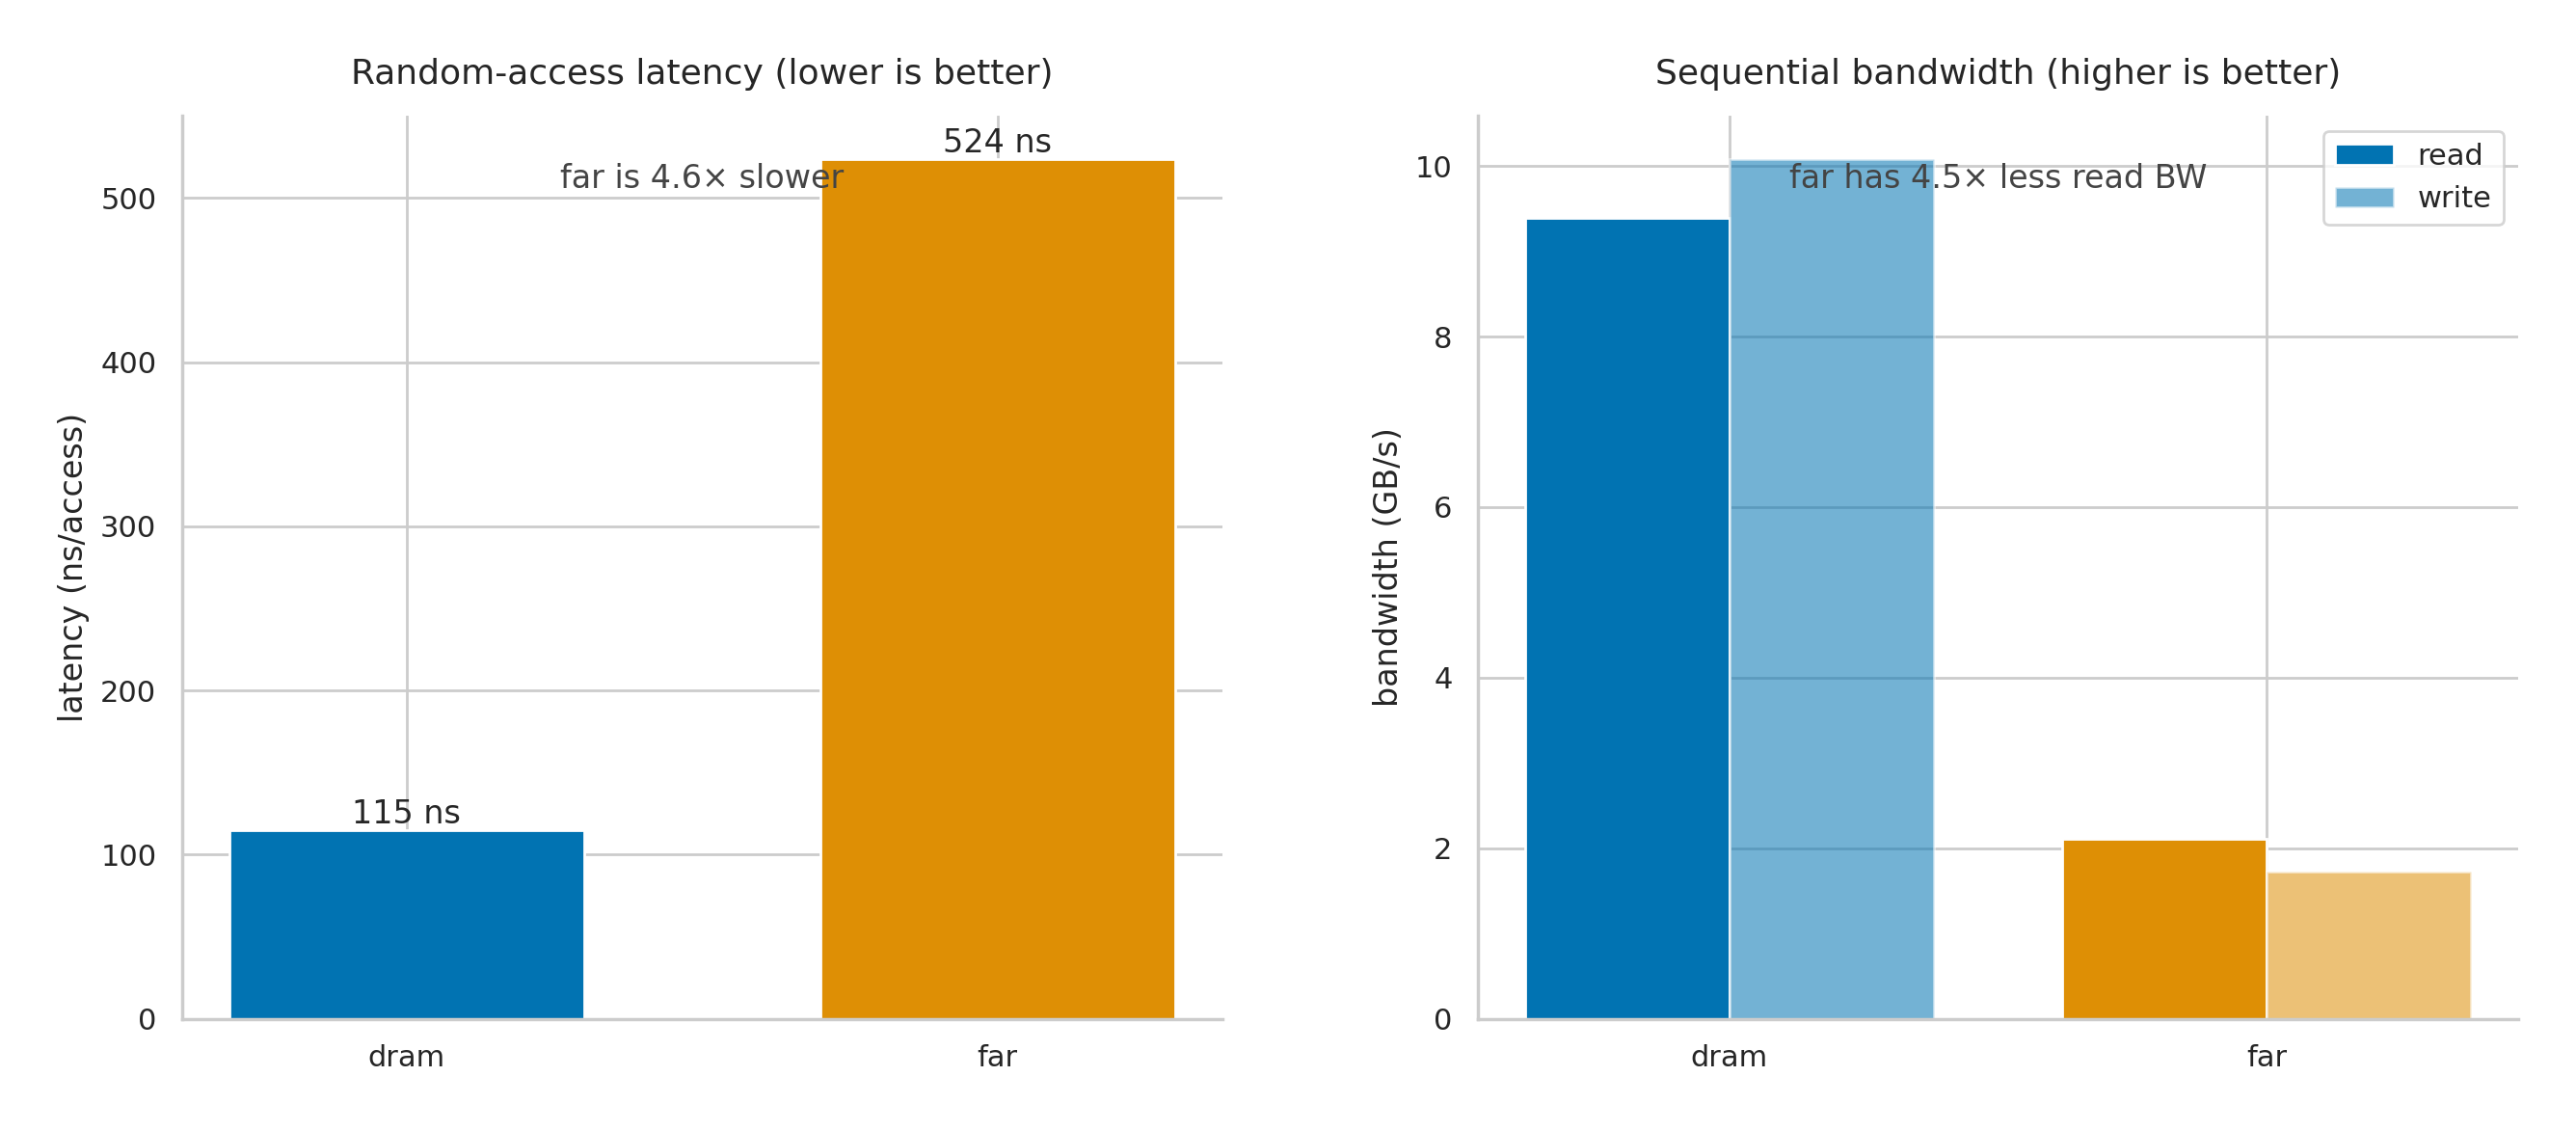
\includegraphics[width=\columnwidth]{fig3_hardware_comparison.png}
  \caption{The two memory tiers genuinely differ. Far memory has $4.6\times$ the
  random-access latency and $\sim\!4.5\times$ less read bandwidth than DRAM.}
  \label{fig:hw}
\end{figure}

\subsection{The framework is free}

With \texttt{all\_dram} the runtime is behaviorally identical to stock OCaml and
we measure no wall-time overhead over an unmodified compiler: the placement seam
is dormant when the policy never sends anything far.

The per-decision cost is the more pointed question, since \texttt{choose\_arena}
fires once per promoted object. Figure~\ref{fig:cost} measures it directly,
reporting the median of 100 runs with interquartile error bars. A decision costs
about $2$~ns when the policy is compiled in, and the \texttt{dlopen}'d loadable
policy costs only a few tenths of a nanosecond more --- the cost of one
well-predicted indirect call. Against a far-access latency of hundreds of
nanoseconds, the decision is effectively free; the framework's flexibility does
not come at the price of a hot-path tax.

\begin{figure}[t]
  \centering
  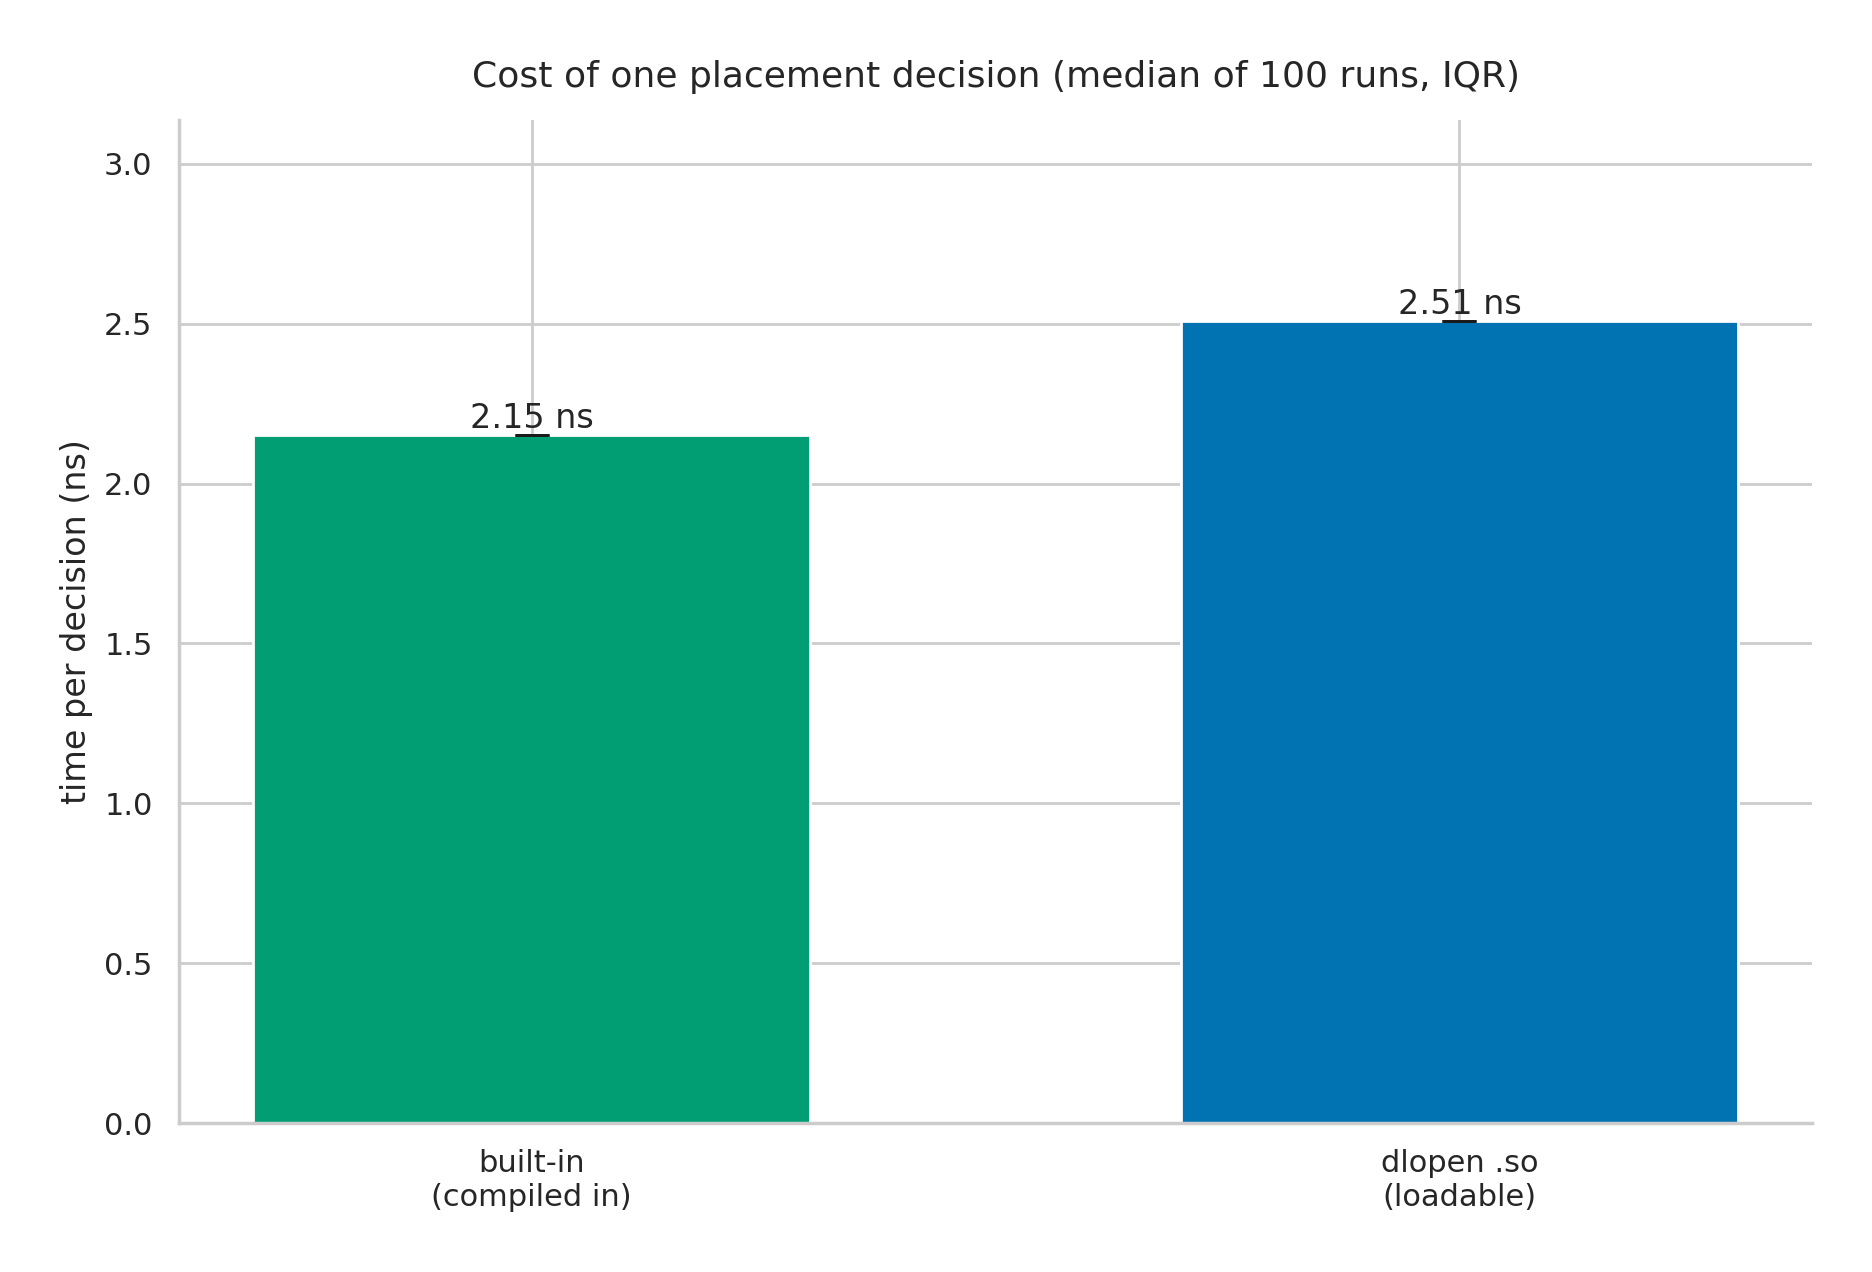
\includegraphics[width=\columnwidth]{fig5_overhead.png}
  \caption{A placement decision costs $\sim\!2$~ns. Making the policy a loadable
  \texttt{dlopen}'d \texttt{.so} rather than a compiled-in built-in adds only the
  cost of one indirect call.}
  \label{fig:cost}
\end{figure}

\subsection{Policies steer, and steering pays under pressure}

The substantive question is whether \emph{which tier an object lands in} matters,
and whether a cheap structural policy can exploit it. We run three workloads ---
\texttt{ptrchase} (pointer chasing, low MLP), \texttt{arraytraverse} (flat array
traversal, high MLP), and a \texttt{mixed} workload --- under a DRAM cap set to
roughly half the working-set footprint, and normalize wall time to the
all-in-DRAM, no-pressure run (Figure~\ref{fig:spread}).

Three behaviors emerge. On \texttt{arraytraverse}, every policy --- including
\texttt{all\_far} --- sits at $\sim\!1.0$: a flat, sequentially streamed,
high-MLP structure tolerates the far tier almost perfectly, so placement barely
matters and even pushing everything far is fine. On the two latency-sensitive
workloads, the spread is wide. For \texttt{mixed}, naive \texttt{all\_far} is
$2.4\times$ slower than the baseline, but \texttt{flat\_far} --- which keeps
pointer-bearing (low-MLP) objects in DRAM and sends only flat objects far ---
lands at $1.08\times$, recovering nearly all of the lost performance, and even
edges out \texttt{all\_dram} under the cap because \texttt{all\_dram} is forced to
spill indiscriminately once DRAM fills. For \texttt{ptrchase},
\texttt{all\_far} is $1.9\times$ slower while a \texttt{size\_threshold} policy
returns essentially to the baseline. In short, the right cheap Tier-0 policy
recovers most of the all-in-DRAM performance, and no single policy is best across
all workloads --- which is precisely the argument for a framework that makes the
policy swappable rather than for one baked-in heuristic.

\begin{figure}[t]
  \centering
  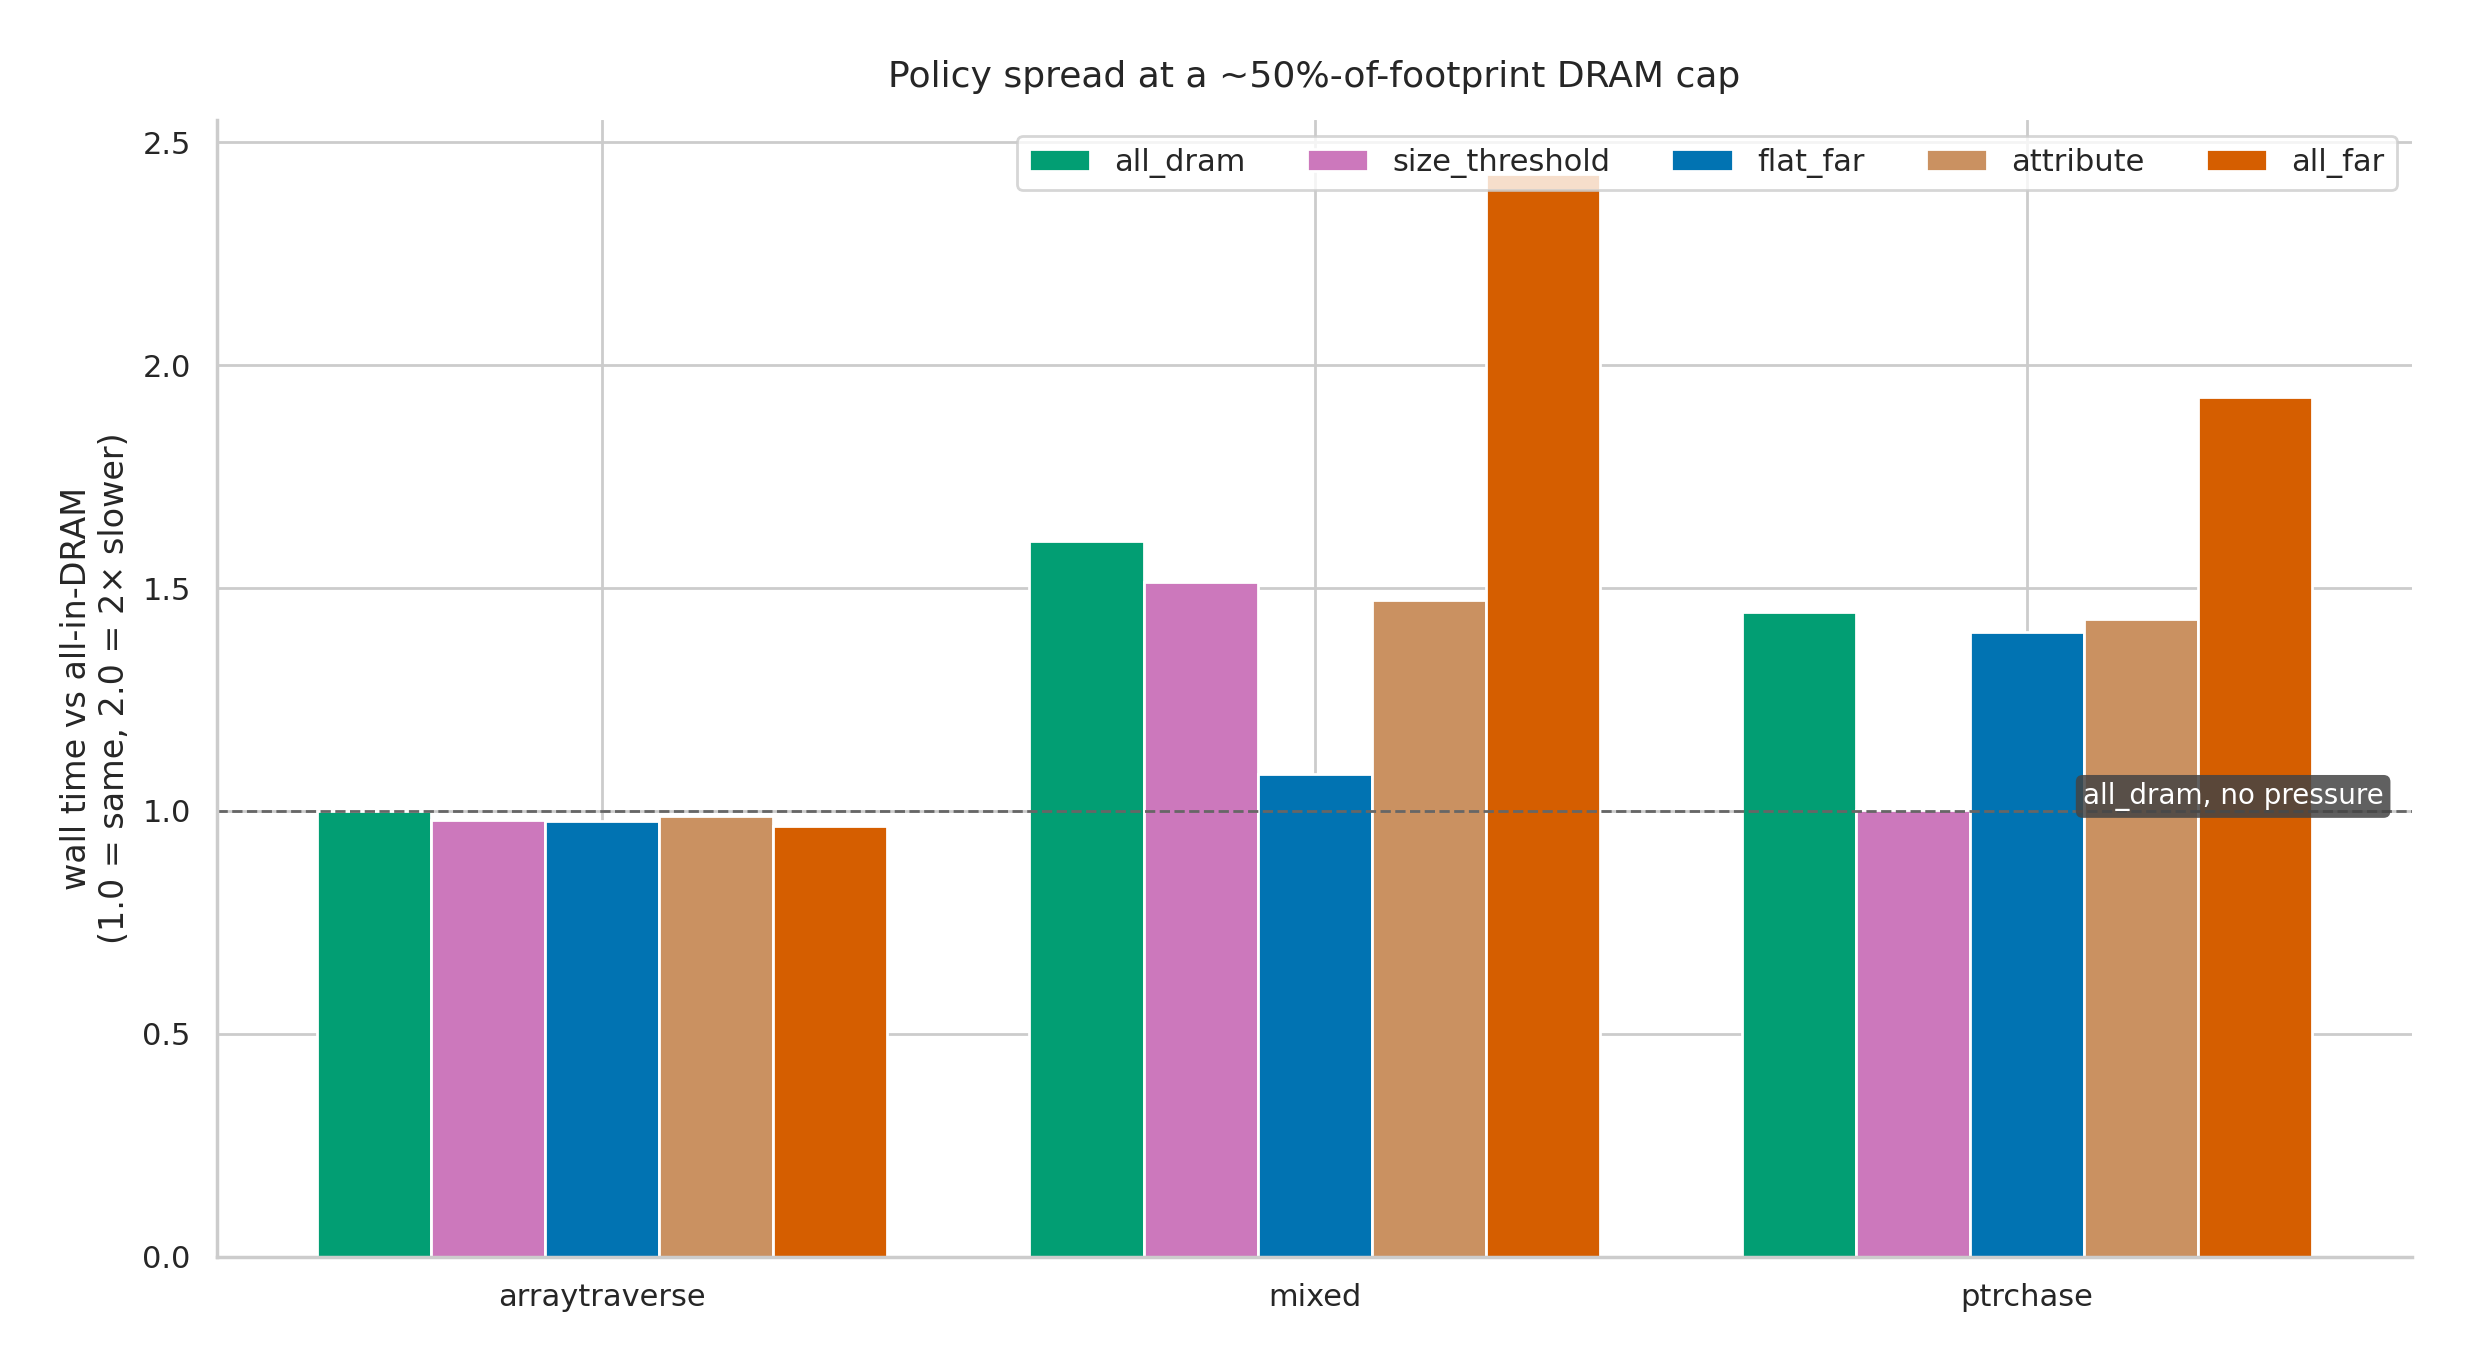
\includegraphics[width=\columnwidth]{fig1_policies_work.png}
  \caption{Policy spread at a $\sim\!50\%$-of-footprint DRAM cap, normalized to
  all-in-DRAM with no pressure (dashed line). Criticality-aware policies
  (\texttt{flat\_far}, \texttt{size\_threshold}) recover most of the envelope on
  latency-sensitive workloads, while naive \texttt{all\_far} is up to $2.4\times$
  slower. On the high-MLP \texttt{arraytraverse}, placement barely matters.}
  \label{fig:spread}
\end{figure}

\subsection{Discussion}

The arena-occupancy accounting confirms the steering is real and not an artifact
of timing noise: occupancy splits between the tiers exactly as each policy
intends. The win, as expected, grows as DRAM grows scarcer --- at a generous cap
the policies converge, and they diverge as the cap tightens and the far tier's
latency is exposed. The \texttt{arraytraverse} result is a useful negative: it
shows the framework is measuring something real (a high-MLP structure is
genuinely indifferent to tier) rather than always rewarding ``more DRAM.''

\section{Related work}

PACT~\cite{pact2026} argues for criticality-first tiered-memory placement but
operates at the OS page level, blind to runtime object structure.
TrackFM~\cite{trackfm2024} provides compiler support for far memory over
unmodified code and therefore works in the middle-end; our attribute path is a
more front-end contribution that lets the programmer state intent directly.
Merchandiser~\cite{merchandiser2023} places data on heterogeneous memory by
hotness and load balance. ALASKA~\cite{alaska2024} highlights object mobility as
the lever managed runtimes have and unmanaged ones lack. We sit one layer below
all of these: rather than ship a placement policy, we ship the runtime
\emph{mechanism} that lets a policy --- built-in, \texttt{dlopen}'d, or expressed
via source attributes --- be written, swapped, and measured at near-zero cost.

\section{Contributions}

\begin{enumerate}
  \item A garbage-collector and runtime patch to OCaml~5 implementing a
  programmable, mechanism/policy-split object-placement framework across tiered
  memory: two arenas, policy-driven promotion routing, per-arena accounting, a
  frozen one-header ABI, built-in policies, and a \texttt{dlopen} loadable-policy
  path.
  \item A compiler front-end patch threading \texttt{[@far\_memory]} /
  \texttt{[@main\_memory]} attributes from source through Lambda and Cmm into the
  object header, with an \texttt{attribute} policy that honors them.
  \item Hand-written benchmarks (pointer-chasing, array-traversal, and mixed)
  with a memory-pressure harness, and an evaluation showing the framework is free
  ($\sim\!2$~ns/decision, no overhead over stock OCaml) and that cheap Tier-0
  policies recover most of the all-in-DRAM performance under pressure.
\end{enumerate}

\section{Conclusion}

Treating GC object placement as a programmable policy --- mechanism in the
runtime, judgment in a swappable pure function --- is both cheap and effective.
The engine defends correctness so the policy never has to, a decision costs a
couple of nanoseconds, and the right structural policy turns a $2.4\times$
far-memory penalty back into near-baseline performance. The framing deliberately
trades the search for one winning heuristic for an apparatus that makes such
heuristics cheap to write, safe to run, and easy to compare --- and leaves
migration, richer features, and an OCaml policy DSL as ABI-ready future work.

\bibliographystyle{ACM-Reference-Format}
\bibliography{references}

\appendix
\section{AI Usage Disclosure}
This was a yes-AI project. Per the project's stated policy, the benchmarks were
written by hand and not AI-generated. AI assistance (Claude) was used elsewhere
in the engineering and in drafting this report; the author has read and reviewed
every part of the contribution and takes responsibility for its quality and
provenance.

\end{document}
